\documentclass[11pt,a4paper]{article}

\usepackage[margin=2.5cm]{geometry}
\usepackage{amsmath,amssymb,amsthm}
\usepackage{stmaryrd}
\usepackage{hyperref}
\usepackage{enumitem}
\usepackage{graphicx}
\usepackage{tikz}
\usepackage{tikz-cd}
\usetikzlibrary{decorations.pathmorphing,calc,fit,backgrounds}

\theoremstyle{definition}
\newtheorem{definition}{Definition}[section]
\newtheorem{example}[definition]{Example}
\newtheorem{remark}[definition]{Remark}

\theoremstyle{plain}
\newtheorem{proposition}[definition]{Proposition}

\newcommand{\Set}{\mathbf{Set}}
\newcommand{\cont}[2]{#1 \triangleleft #2}
\newcommand{\Ext}[1]{\llbracket #1 \rrbracket}
\newcommand{\Free}{\mathrm{Free}}

\title{\textbf{Two-Coloured Trees, Container Composition,\\
and Compiler Intermediate Representations}}
\author{Robin Langer \\ \small For discussion with Neil Ghani}
\date{July 2026}

\begin{document}
\maketitle

\begin{abstract}
We observe that the composition of containers (Abbott--Altenkirch--Ghani)
produces trees with two structurally distinct kinds of edge: \emph{outer}
edges connecting nodes in the composite tree, and \emph{inner} edges
encoding the structure within each node. When the composition is iterated
to arbitrary depth, we obtain the free monad on the container functor.
We apply this perspective to compiler intermediate representations (IRs),
where the two colours correspond to \emph{term structure} (how subterms
compose) and \emph{binding structure} (how variables come into scope).
Compilation passes become container morphisms, and administrative
normal form (ANF) conversion is monad multiplication---collapsing one
colour into the other.
\end{abstract}

%% ===================================================================
\section{The Diagram}
%% ===================================================================

The following diagram shows a tree with two colours of edge. Outer edges
(solid lines) connect nodes. Inner structure (circles nested within circles)
encodes the shape at each node---its positions and internal wiring. Each
innermost circle is a \emph{port}: a position where an outer edge attaches
to a child.

\begin{center}
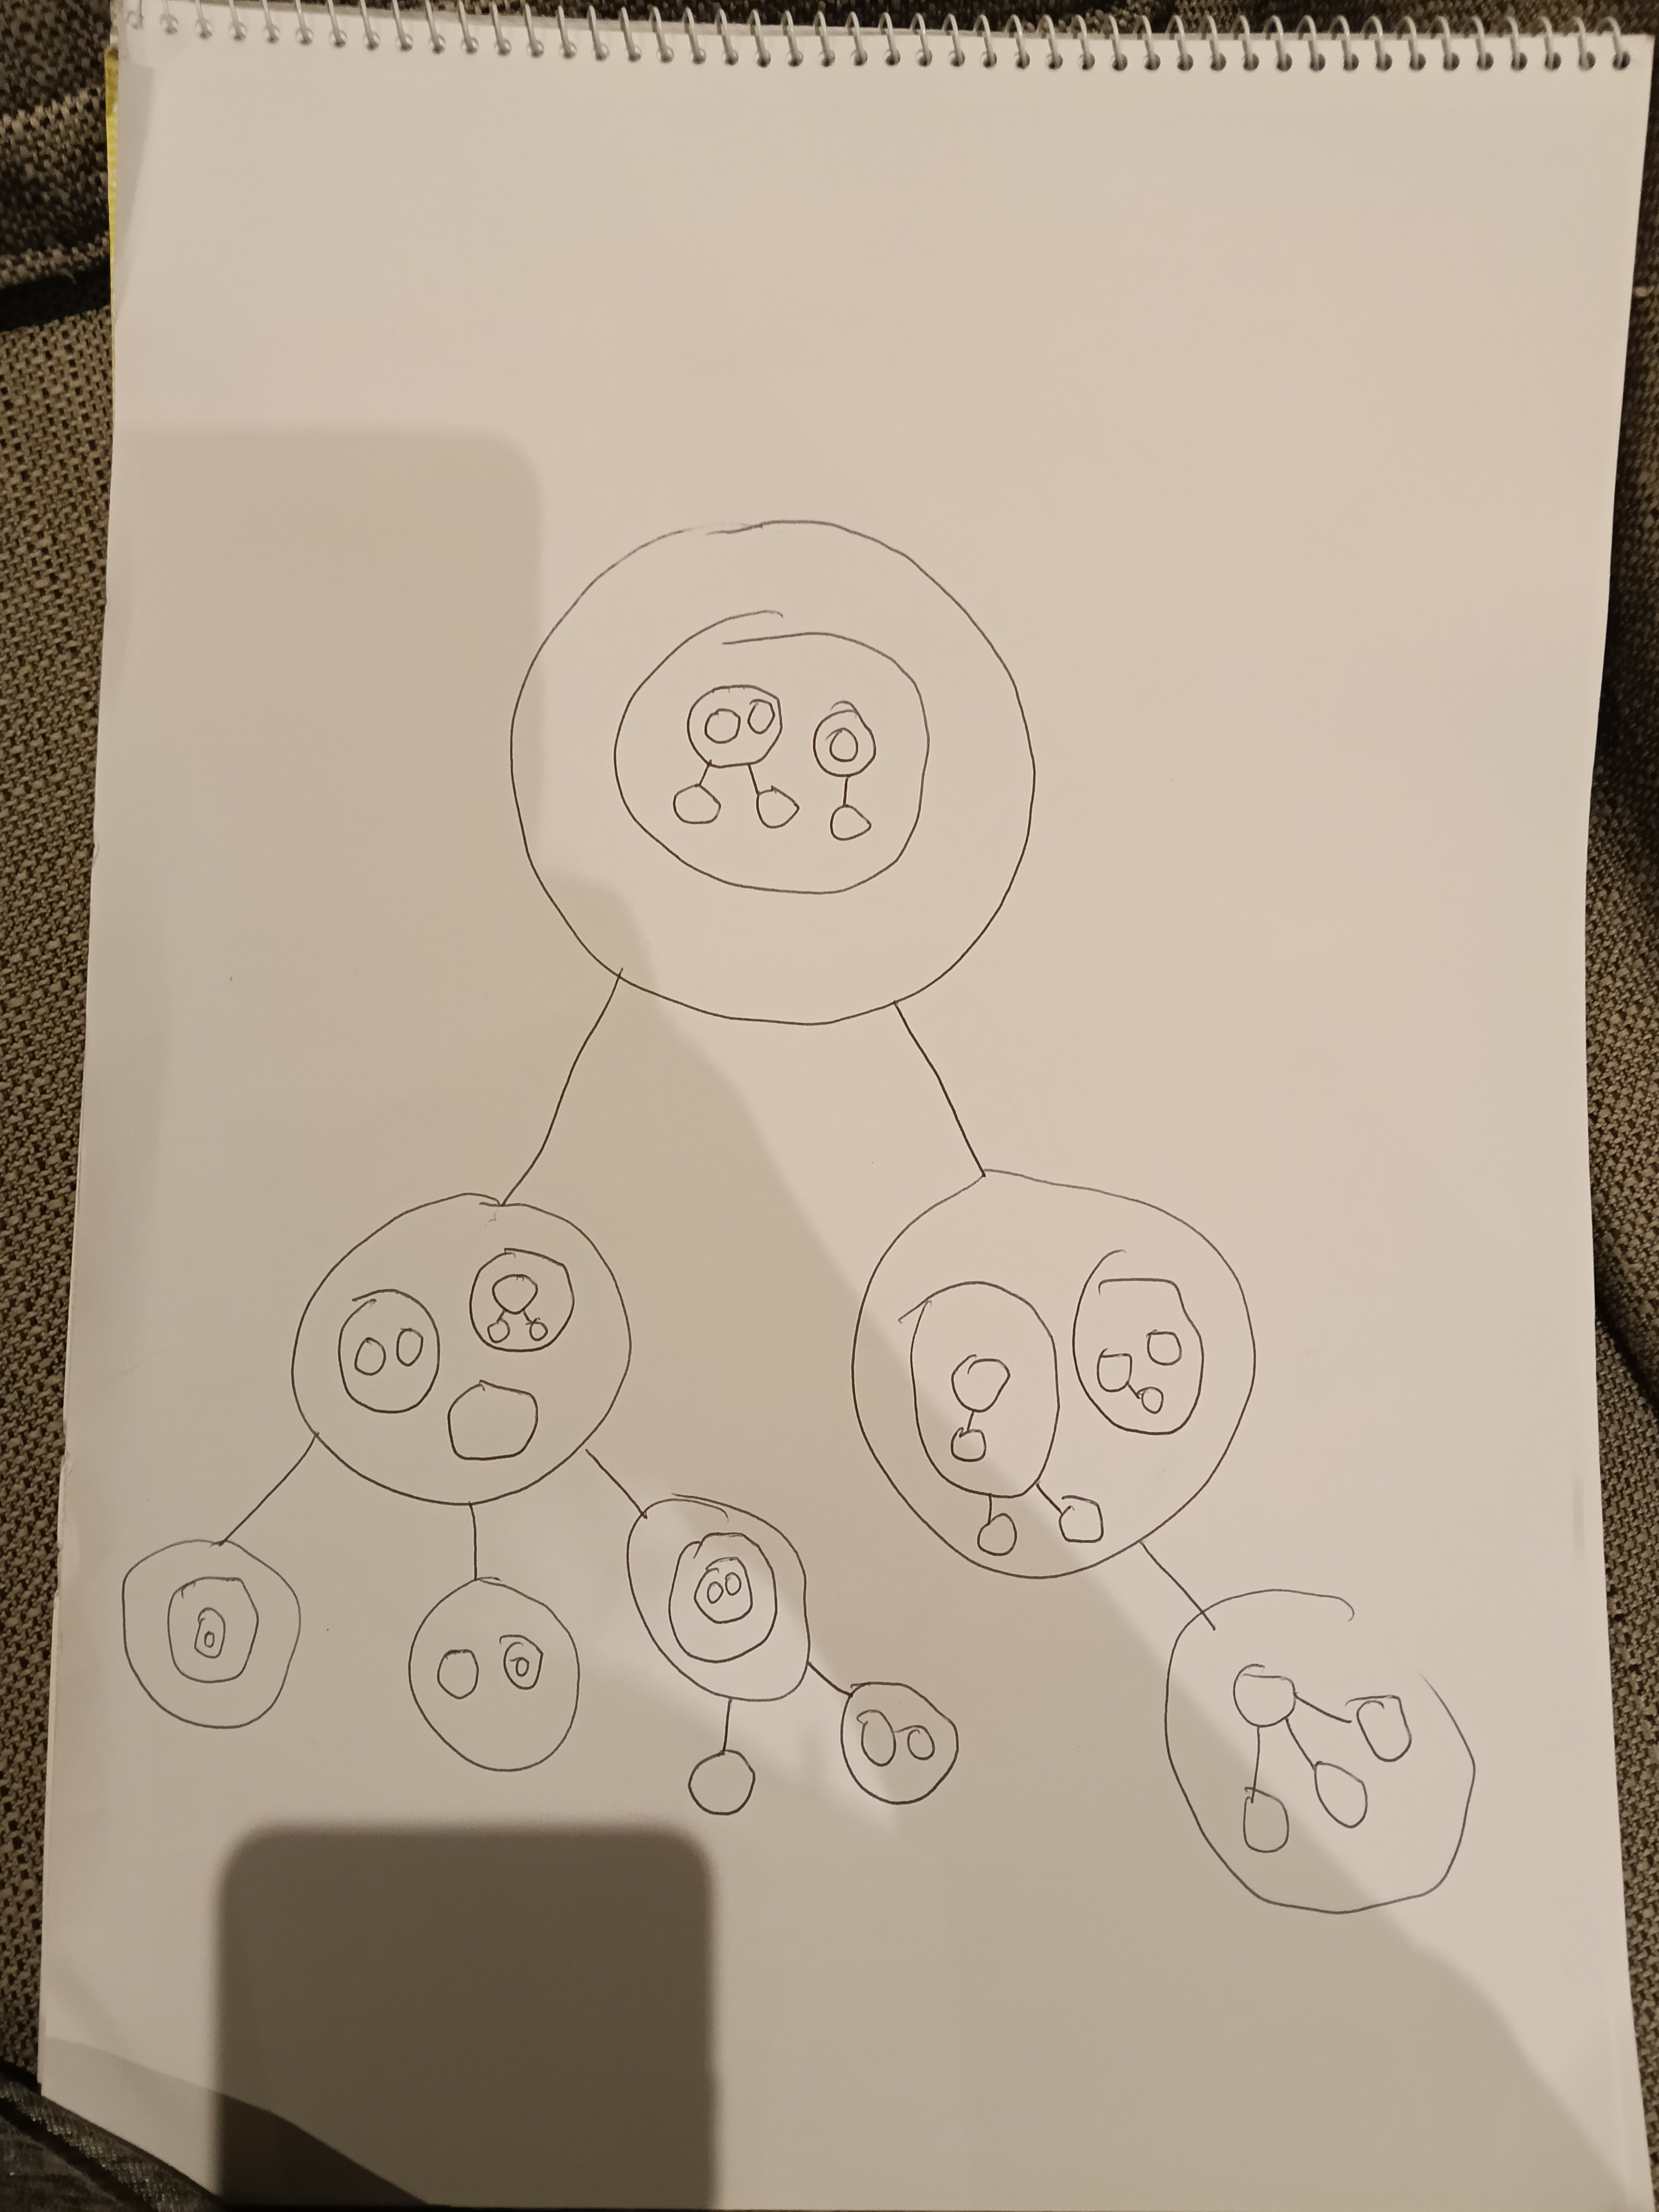
\includegraphics[width=0.55\textwidth]{two-colour-tree.jpg}
\end{center}

The diagram has two kinds of structural relationship:
\begin{enumerate}[nosep]
\item \textbf{Outer edges} (solid lines between circles): the tree structure
  connecting nodes to children. These are the positions of the \emph{outer}
  container.
\item \textbf{Inner structure} (circles nested within circles, connected by
  thin lines): the internal wiring of each node. The leaves (ports) of the
  inner tree are the positions where outer edges attach.
\end{enumerate}

%% ===================================================================
\section{Container Composition Produces Two Colours}
%% ===================================================================

Recall that a container $\cont{S}{P}$ is a set $S$ of shapes with a
family of positions $P : S \to \Set$, and its extension is
\[
\Ext{\cont{S}{P}}(X) = \coprod_{s \in S} X^{P(s)}.
\]

\begin{definition}[Composition of containers]
Given containers $C_1 = \cont{S_1}{P_1}$ and $C_2 = \cont{S_2}{P_2}$,
their composition $C_1 \circ C_2$ is the container with:
\begin{itemize}[nosep]
\item Shapes: $\displaystyle \coprod_{s_1 \in S_1}
  S_2^{\,P_1(s_1)}$
  \quad (an outer shape $s_1$ plus a choice of inner shape at each outer
  position),
\item Positions at shape $(s_1, v)$: $\displaystyle \coprod_{p \in P_1(s_1)}
  P_2(v(p))$
  \quad (an outer position $p$ plus an inner position at $v(p)$).
\end{itemize}
Its extension satisfies
$\Ext{C_1 \circ C_2} \cong \Ext{C_1} \circ \Ext{C_2}$.
\end{definition}

The shape of a composite element is a \textbf{tree of depth~2}: an outer
shape $s_1$ whose positions are filled with inner shapes $v(p) \in S_2$.
The two colours in the diagram are exactly the two levels of this
nesting:
\begin{itemize}[nosep]
\item Colour~1 (outer edges) corresponds to the outer positions $p \in P_1(s_1)$.
\item Colour~2 (inner structure) corresponds to the inner positions
  $q \in P_2(v(p))$.
\end{itemize}

\begin{remark}
In the diagram, the self-similar structure---inner nodes themselves
containing structure---suggests more than two levels. This is the
iterated composition $C^n$, or in the limit, the \emph{free monad}.
\end{remark}

%% ===================================================================
\section{The Free Monad: Arbitrary Depth}
%% ===================================================================

If $C$ is a container, its free monad $\Free(C)$ is the container whose
elements are \emph{finite trees of arbitrary depth} over $C$:
\[
\Free(C)(X) = X + C(\Free(C)(X))
\]
or equivalently, as a W-type (well-founded tree type):
\[
\Free(C)(X) = \mu T.\; X + \coprod_{s \in S} T^{P(s)}.
\]
An element is either a leaf labelled by $x \in X$, or a node with shape $s$
and a child at each position. The number of ``colours'' is the depth of the
tree: a path from root to leaf passes through $n$ node boundaries (each a
colour-transition), where $n$ varies across branches.

The monad structure is:
\begin{itemize}[nosep]
\item \textbf{Unit} $\eta : X \to \Free(C)(X)$: embed $x$ as a leaf.
\item \textbf{Multiplication} $\mu : \Free(C)(\Free(C)(X)) \to \Free(C)(X)$:
  given a tree whose leaves are themselves trees, \emph{graft} the leaf-trees
  onto the outer tree. This \textbf{dissolves one level of nesting}---it
  merges two adjacent colours into one.
\end{itemize}

The diagram on the first page, with its self-similar nesting, is an element
of $\Free(C)(X)$ for some $C$---a tree of trees of trees, with $\mu$ unapplied.

%% ===================================================================
\section{The Metacircular Evaluator}
%% ===================================================================

The purest example of a two-coloured tree---and the composition it
embodies---is a Lisp interpreter written in Lisp.

\subsection{S-Expressions as Labelled Rose Trees}

Let $A$ be a set of \emph{labels}---numbers, symbols, booleans,
the empty list \texttt{nil}, and any other atomic data the language
supports. The \textbf{labelled rose tree container} is:
\[
C = \cont{A \times \mathbb{N}}{P} \quad\text{where}\quad
P(a, n) = \{0, 1, \ldots, n-1\}.
\]
A shape $(a, n)$ is a node labelled $a \in A$ with $n$ children.
Leaves are nodes with $n = 0$. The extension is
\[
\Ext{C}(X) = \coprod_{(a,n)} X^n \;\cong\; A \times \mathrm{List}(X).
\]
The free monad on this container is the type of S-expressions:
\[
T(X) = \Free(C)(X) = \mu R.\; X + A \times \mathrm{List}(R).
\]
An S-expression is either a variable ($x \in X$) or a labelled node
with a list of children, each recursively an S-expression. Every node
in the tree---leaf or internal---carries a label from $A$. The
expression \texttt{(+ 1 2)} is a node labelled $\mathord{+}$ with
two children labelled $1$ and $2$:
\begin{center}
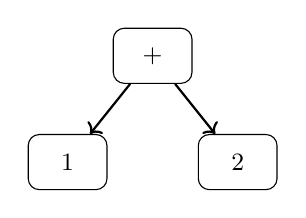
\begin{tikzpicture}[
    node/.style={draw, rounded corners, minimum width=10mm, minimum height=7mm,
      font=\small},
    arr/.style={thick, ->},
    scale=0.9
  ]
  \node[node] (plus) at (0,0) {$+$};
  \node[node] (one) at (-1.2,-1.5) {$1$};
  \node[node] (two) at (1.2,-1.5) {$2$};
  \draw[arr] (plus) -- (one);
  \draw[arr] (plus) -- (two);
\end{tikzpicture}
\end{center}
The label $\mathord{+}$ is \emph{on} the node, not in a child
position. Arity is part of the shape: $(\mathord{+}, 2)$ says
``labelled $+$, two children.'' The labels are what the evaluator's
algebra will pattern-match on.

\begin{remark}[Lisp's encoding]
Traditional Lisp represents S-expressions as unlabelled binary cons
cells, encoding the labelled rose tree \texttt{(+ 1 2)} as the
cons-chain \texttt{(+ . (1 . (2 . nil)))}. This is the classical
first-child/next-sibling encoding of a rose tree as a binary tree.
The container $A \sqcup \{\mathsf{cons}\}$ with $P(\mathsf{cons})
= \{0,1\}$ describes this encoding; the container $A \times \mathbb{N}$
describes the intended tree. The catamorphism must reconstruct the
labelled-node structure from the cons-chain---the algebra recovers
what the encoding hides.
\end{remark}

\subsection{The Metacircular Evaluator is Self-Composition}

A Lisp interpreter written in Lisp is itself an element of
$T = \Free(C)$---a labelled rose tree. The program it interprets is
another element of $T$. When the interpreter receives a program as
quoted data, the combined object is an element of the
\textbf{container composition} $T \circ T$: a labelled rose tree
whose data-positions contain labelled rose trees.

The two colours are:
\begin{itemize}[nosep]
\item \textbf{Colour~1} (outer tree): the interpreter's own
  structure---its \texttt{eval}, \texttt{apply}, \texttt{cond}
  dispatch.
\item \textbf{Colour~2} (inner trees): the program fragments sitting
  at the data-positions of the interpreter, received via \texttt{quote}.
\end{itemize}

\begin{center}
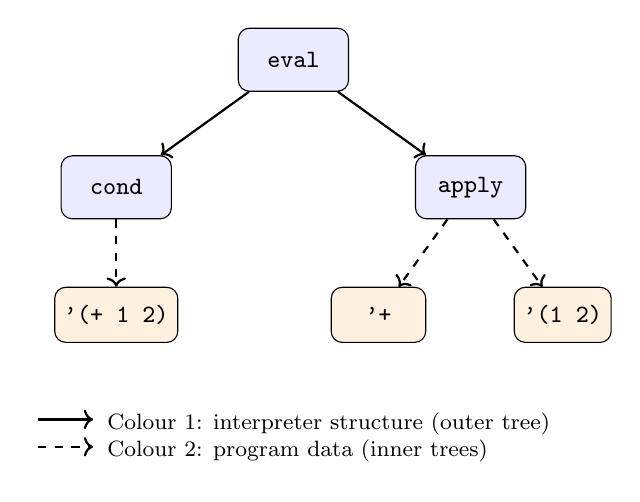
\begin{tikzpicture}[
    outer/.style={draw, rounded corners, minimum width=14mm,
      minimum height=8mm, font=\small, fill=blue!8},
    inner/.style={draw, rounded corners, minimum width=12mm,
      minimum height=7mm, font=\small, fill=orange!12},
    c1/.style={thick, ->},
    c2/.style={thick, ->, dashed},
    scale=0.9
  ]
  \node[outer] (eval) at (0,0) {\texttt{eval}};
  \node[outer] (cond) at (-2.5,-1.8) {\texttt{cond}};
  \node[outer] (apply) at (2.5,-1.8) {\texttt{apply}};

  \node[inner] (prog) at (-2.5,-3.6) {\texttt{'(+ 1 2)}};
  \node[inner] (fn) at (1.2,-3.6) {\texttt{'+}};
  \node[inner] (args) at (3.8,-3.6) {\texttt{'(1 2)}};

  \draw[c1] (eval) -- (cond);
  \draw[c1] (eval) -- (apply);
  \draw[c2] (cond) -- (prog);
  \draw[c2] (apply) -- (fn);
  \draw[c2] (apply) -- (args);

  \node[font=\footnotesize, anchor=north] at (0, -4.8) {
    \begin{tabular}{@{}l@{\;\;}l@{}}
    \tikz\draw[thick, ->] (0,0) -- (0.7,0); & Colour 1: interpreter
      structure (outer tree) \\
    \tikz\draw[thick, ->, dashed] (0,0) -- (0.7,0); & Colour 2: program
      data (inner trees) \\
    \end{tabular}
  };
\end{tikzpicture}
\end{center}

Because homoiconicity gives $C = C$ on both sides, the composition is
\textbf{self-composition}: $T \circ T = T^2$. The metacircular tower
\[
T \circ T \circ T = T^3
\qquad\text{(interpreter interpreting an interpreter interpreting a
  program)}
\]
iterates the same composition, and in the limit $\Free(C)$ gives $T^*$
---arbitrary depth.

\medskip
\noindent\textbf{Quote constructs the composition.}\quad
The expression \texttt{(eval '(+ 1 2))} is syntactically a single tree
in $T$. The decomposition into $T(T(X))$ requires a boundary between
outer and inner, and that boundary is \textbf{quote}.

An element of $T(T(X))$ is an outer tree whose leaves are filled with
inner trees. The interpreter's code is the outer tree. Its leaves are
of two kinds:
\begin{itemize}[nosep]
\item \textbf{Quoted positions}: the leaf is filled with a non-trivial
  inner tree---a program fragment received as data. In
  \texttt{(eval '(+ 1 2))}, the hole where \texttt{'(+ 1 2)} sits is
  such a leaf, and the inner tree is $(\mathord{+}, [1, 2])$.
\item \textbf{Unquoted positions}: variable references like
  \texttt{env}, calls to \texttt{lookup}, numeric constants. These are
  filled with $\eta(x)$---the monad unit, embedding a single variable
  as a trivial (one-leaf) inner tree.
\end{itemize}
Without quote, every inner tree is trivial ($\eta(x)$), and the
composition collapses: $\mu \circ \eta = \mathrm{id}$, so $T(T(X))$
reduces to $T(X)$---a single colour. Quote is the operation that
\emph{creates} non-trivial inner trees, making the composition
genuinely two-coloured. It is the constructor of $T \circ T$.

\subsection{Evaluation Folds the Composite Tree}

The composition $T \circ T$ gives the \emph{structure} of the
metacircular evaluator. The \emph{semantics} is a fold.

It is tempting to identify evaluation with the monad multiplication
$\mu : T^2 \to T$, but $\mu$ is \emph{grafting}: it splices inner
trees into the outer tree's leaf positions, producing a single tree
without interpreting anything. In Lisp, grafting is quasiquote
with unquote:
\[
\texttt{`(a ,(+ 1 2) c)}
\quad\longrightarrow\quad
\texttt{(a 3 c)}.
\]
The subexpression \texttt{(+ 1 2)} is evaluated \emph{before}
grafting; the graft itself just splices the result in. Grafting is
structural; evaluation is semantic.

\medskip
\noindent\textbf{Eval is a catamorphism.}\quad
Given an algebra
\[
\alpha : A \times \mathrm{List}(V) \;\longrightarrow\; V
\]
mapping each labelled node applied to already-evaluated children to a
value, the catamorphism $\mathrm{cata}(\alpha) : T(X) \to V$ folds the
tree bottom-up:
\begin{itemize}[nosep]
\item \textbf{Variable} ($x \in X$): look up $x$ in the environment.
\item \textbf{Leaf} $(a, [\ ])$: return the value of atom $a$
  (a number returns itself; a symbol is looked up).
\item \textbf{Node} $(a, [v_1, \ldots, v_n])$: apply the semantics
  for label $a$ to the already-folded children $v_1, \ldots, v_n$.
\end{itemize}
The tree is \emph{consumed}, not rearranged. The output is a value in
$V$, not another S-expression:
\begin{center}
\renewcommand{\arraystretch}{1.3}
\begin{tabular}{@{}lll@{}}
\hline
& $\mu$ (grafting) & $\mathrm{cata}(\alpha)$ (eval) \\
\hline
Type & $T^2(X) \to T(X)$ & $T(X) \to V$ \\
Output & another tree & a value \\
Knows about labels? & no & yes (via the algebra $\alpha$) \\
$(\mathord{+},\, [1,\, 2]) \;\mapsto$ & $(\mathord{+},\, [1,\, 2])$
  & $3$ \\
\hline
\end{tabular}
\end{center}

\subsection{Compilation is Also Self-Composition}

A Lisp \emph{compiler} written in Lisp has the same two-coloured
structure: the compiler is an element of $T$, the source program is
an element of $T$, and the combined object is $T \circ T$. The
difference is the operation on the composite tree.

Where interpretation folds to \emph{values} ($T \to V$), compilation
folds to \emph{target trees} ($T \to T_{\mathrm{target}}$). The new
ingredient is a \textbf{container morphism}
$m = (u, f^\sharp) : C \to C_{\mathrm{target}}$:
\begin{itemize}[nosep]
\item \textbf{Forward on shapes} $u : A \times \mathbb{N} \to
  A' \times \mathbb{N}'$: translate each labelled node. A node
  $(\mathsf{lambda}, 2)$ might become $(\mathsf{closure}, 3)$ in
  the target.
\item \textbf{Backward on positions} $f^\sharp : P'(u(s)) \to P(s)$:
  for each child position in the output node, say which child of the
  input node it came from. This is \textbf{provenance}.
\end{itemize}
Lifting $m$ through the free monad yields a tree transformation
$\mathrm{cata}(m) : \Free(C) \to \Free(C_{\mathrm{target}})$: each
source node is translated (forward), its children are recursively
compiled, and provenance (backward) records where everything came from.

The three operations on $T \circ T$ are:
\begin{center}
\renewcommand{\arraystretch}{1.3}
\begin{tabular}{@{}llll@{}}
\hline
Operation & Type & Output & Provenance \\
\hline
$\mu$ (graft) & $T^2 \to T$ & tree & trivial \\
$\mathrm{cata}(\alpha)$ (interpret) & $T \to V$ & values & none \\
$\mathrm{cata}(m)$ (compile) & $T \to T_{\mathrm{tgt}}$ &
  target tree & backward map $f^\sharp$ \\
\hline
\end{tabular}
\end{center}

When the target language is Lisp itself ($C_{\mathrm{target}} = C$),
the morphism is an \textbf{endomorphism} $m : C \to C$ and the
catamorphism is an endofunction $\mathrm{cata}(m) : T \to T$. The
compiler can then be applied to its own source code---\textbf{%
bootstrapping}. This is a second consequence of homoiconicity: not
just the interpreter folding its own description (metacircularity),
but the compiler transforming its own source (self-hosting).

\subsection{Homoiconicity is the Self-Composition Condition}

Most languages have $T_1 \circ T_2$: the tool (interpreter or
compiler) is a tree of type $T_1$, the target program is a tree of
type $T_2$. This is composition of \emph{different} containers.

Homoiconicity means $T_1 = T_2 = T$: the composition becomes
$T \circ T = T^2$. The fold (whether to values or to target trees)
is itself an element of $T$, so it can be applied to a description of
itself. This is the self-composition condition: the same labelled rose
tree container on both sides.

\begin{remark}
Non-homoiconic languages can still have interpreters and compilers,
but the fold's algebra must bridge two different containers via a
container morphism $(u, f^\sharp) : C_{\text{source}} \to
C_{\text{target}}$. Only when $C_{\text{source}} =
C_{\text{target}}$ is the composition self-composition, and only
then can the tool process a representation of itself.
\end{remark}

%% ===================================================================
\section{Snoc-Trees and Composition}
%% ===================================================================

The two-coloured tree has a natural directional asymmetry: colour-1
edges branch (a node may have many children), while colour-2 edges
are sequential (each binding extends the context by one variable).
The colour-2 spine is a \emph{snoc-list}.

\subsection{Snoc-Lists as Containers}

A \textbf{snoc-list} builds rightward by appending:
\[
\mathsf{Lin} \mathbin{{:}{>}} a_1 \mathbin{{:}{>}} a_2
  \mathbin{{:}{>}} a_3
\qquad\text{(three elements, built right-to-left)}
\]
As a container, the snoc-list functor $L$ has:
\begin{itemize}[nosep]
\item Shapes $S = \mathbb{N}$ (the length).
\item Positions at shape $n$: $P(n) = \{0, 1, \ldots, n-1\}$ (slots
  indexed from the right, matching de~Bruijn convention: position~0
  is the most recently appended element).
\end{itemize}
Its extension is $\Ext{L}(X) = \coprod_{n \geq 0} X^n$---finite
sequences, the same as the list container but with the opposite
construction bias.

\subsection{Contexts are Snoc-Lists}

In dependent type theory, a typing context is a snoc-list of typed
variable declarations:
\[
\Gamma = (\cdot \mathbin{{:}{>}} (x_1 : A_1) \mathbin{{:}{>}}
  (x_2 : A_2(x_1)) \mathbin{{:}{>}} (x_3 : A_3(x_1, x_2))).
\]
Each ${:}{>}$ is a colour-2 edge in the two-coloured tree. A path from
the root of the AST to a node, reading only the binding edges (colour~2)
encountered along the way, yields the snoc-list context at that node.
Colour-1 edges do not change the context; colour-2 edges snoc onto it.

\begin{center}
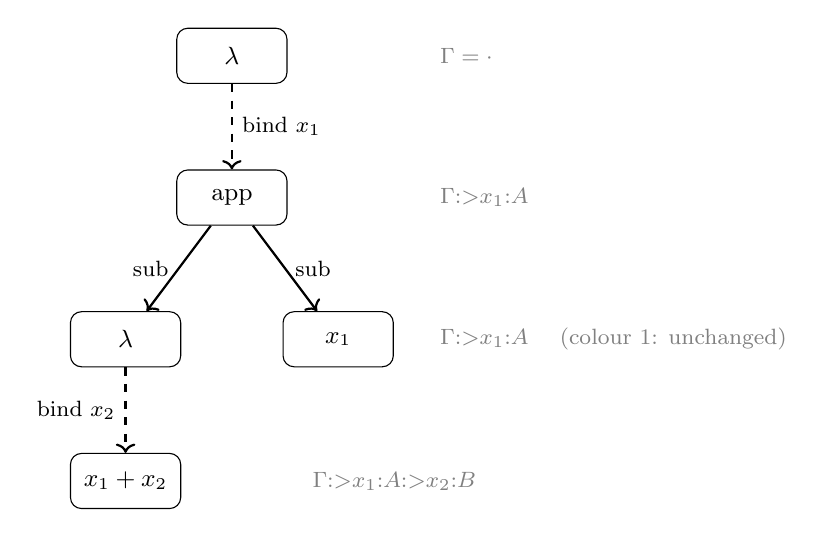
\begin{tikzpicture}[
    node/.style={draw, rounded corners, minimum width=14mm, minimum height=7mm,
      font=\small},
    c1/.style={thick, ->},
    c2/.style={thick, ->, dashed},
    ctx/.style={font=\footnotesize, text=gray, anchor=west},
    scale=0.9
  ]
  % Nodes
  \node[node] (lam1) at (0,0) {$\lambda$};
  \node[node] (app) at (0,-2) {app};
  \node[node] (lam2) at (-1.5,-4) {$\lambda$};
  \node[node] (var) at (1.5,-4) {$x_1$};
  \node[node] (body) at (-1.5,-6) {$x_1 + x_2$};

  % Edges
  \draw[c2] (lam1) -- node[right, font=\footnotesize] {bind $x_1$} (app);
  \draw[c1] (app) -- node[left, font=\footnotesize] {sub} (lam2);
  \draw[c1] (app) -- node[right, font=\footnotesize] {sub} (var);
  \draw[c2] (lam2) -- node[left, font=\footnotesize] {bind $x_2$} (body);

  % Context annotations
  \node[ctx] at (2.8, 0) {$\Gamma = \cdot$};
  \node[ctx] at (2.8, -2) {$\Gamma {:}{>} x_1{:}A$};
  \node[ctx] at (2.8, -4) {$\Gamma {:}{>} x_1{:}A$ \quad (colour 1: unchanged)};
  \node[ctx] at (1, -6) {$\Gamma {:}{>} x_1{:}A {:}{>} x_2{:}B$};
\end{tikzpicture}
\end{center}

The snoc-list at each node is the \emph{accumulated} colour-2 path.
De~Bruijn index~0 refers to the most recent ${:}{>}$ (the last binding
edge crossed). This is why snoc-lists are the natural representation:
access to the most recent element is $O(1)$, matching the frequency
with which bound variables are used near their binders.

\subsection{Composition of Snoc-Trees}

A \textbf{snoc-tree} is a tree built by iterated snoc---equivalently,
it is the free monad on the snoc-list container. But the interesting
composition is not snoc-list with snoc-list; it is \emph{snoc-list
composed with a branching container}. This is exactly the two-coloured tree.

Let $B = \cont{S_B}{P_B}$ be a branching container (the syntax:
shapes are constructors, positions are argument slots) and let
$L = \cont{\mathbb{N}}{[n]}$ be the snoc-list container. The
composition $B \circ L$ has:
\begin{itemize}[nosep]
\item Shapes: a syntax constructor $s \in S_B$ together with, at each
  position $p \in P_B(s)$, a natural number $n_p$ (the length of the
  snoc-list---how many bindings this edge introduces).
\item Positions at shape $(s, \{n_p\})$: $\coprod_{p \in P_B(s)} [n_p]$
  (an argument slot $p$ plus a de~Bruijn index within the $n_p$ new
  bindings at that slot).
\end{itemize}
An element of $\Ext{B \circ L}(X)$ is a syntax node where each argument
slot carries a \emph{telescope} of new bindings before reaching the child
term. This is precisely the standard notion of a syntax constructor in
dependently typed languages: each argument may bind zero or more variables
before the subterm.

\begin{example}[The $\Pi$-type constructor]
The shape is $\Pi$ with two positions: the domain and the codomain.
The domain binds nothing ($n_1 = 0$); the codomain binds one variable
($n_2 = 1$). So the composite shape is $(\Pi, [0, 1])$, and the positions
are $\{(\text{dom}, \varnothing)\} \cup \{(\text{cod}, 0)\}$---the domain
has no new de~Bruijn indices, the codomain introduces index~0.
\end{example}

\begin{example}[Telescopic binders]
A dependent record type with fields
$\{(x_1 : A_1),\; (x_2 : A_2(x_1)),\; (x_3 : A_3(x_1, x_2))\}$
has a single position with $n = 3$. The three bindings form a snoc-list
$\cdot \mathbin{{:}{>}} x_1 \mathbin{{:}{>}} x_2 \mathbin{{:}{>}} x_3$,
and the positions within this telescope are de~Bruijn indices $\{0, 1, 2\}$.
The whole structure is one element of $B \circ L$.
\end{example}

The composition $L \circ B$ goes the other way: a snoc-list whose elements
are trees. This is a \textbf{sequence of compilation passes}---each
element of the snoc-list is an IR tree, appended in order. The most
recent pass (index~0) is the current IR; earlier passes are history. The
snoc structure gives $O(1)$ access to the current state while preserving
the full provenance chain.

\medskip
\noindent\textbf{The monad multiplication.}\quad
For $B \circ L$, the multiplication $\mu : (B \circ L) \circ (B \circ L)
\to B \circ L$ concatenates telescopes. If a binding introduces a
telescope $\Delta_1$, and within that scope another binding introduces
$\Delta_2$, flattening merges them:
\[
\Delta_1 \mathbin{{:}{>}} \Delta_2 \quad\longrightarrow\quad
\Delta_1 \mathbin{+\!+} \Delta_2.
\]
This is the \texttt{let}-flattening operation of ANF, generalised from
single bindings to telescopes: nested scopes are concatenated into a
single snoc-list of bindings.

%% ===================================================================
\section{Application to Compiler Theory}
%% ===================================================================

Compiler intermediate representations are trees. The container perspective
makes the \emph{two-colour structure} of these trees explicit, and gives
precise meaning to compilation passes and normal forms.

\subsection{Syntax Trees Have Two Colours}

The abstract syntax tree (AST) of a dependently typed language has two
structurally distinct kinds of descent:

\begin{center}
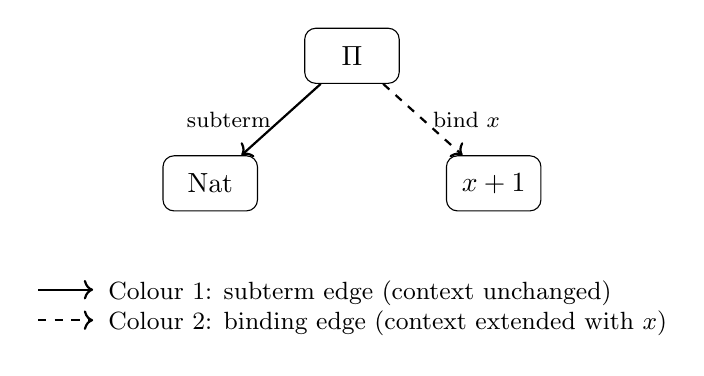
\begin{tikzpicture}[
    node/.style={draw, rounded corners, minimum width=12mm, minimum height=7mm},
    blue edge/.style={thick, ->},
    red edge/.style={thick, ->, dashed},
    scale=0.9
  ]
  \node[node] (pi) at (0,0) {$\Pi$};
  \node[node] (nat) at (-2,-1.8) {Nat};
  \node[node] (plus) at (2,-1.8) {$x + 1$};

  \draw[blue edge] (pi) -- node[left, font=\footnotesize] {subterm} (nat);
  \draw[red edge] (pi) -- node[right, font=\footnotesize] {bind $x$} (plus);

  \node[anchor=north, font=\small] at (0, -3) {
    \begin{tabular}{@{}l@{\;\;}l@{}}
    \tikz\draw[thick, ->] (0,0) -- (0.7,0); & Colour 1: subterm edge
      (context unchanged) \\
    \tikz\draw[thick, ->, dashed] (0,0) -- (0.7,0); & Colour 2: binding edge
      (context extended with $x$) \\
    \end{tabular}
  };
\end{tikzpicture}
\end{center}

\begin{itemize}[nosep]
\item \textbf{Colour~1} (subterm edges): descend into a subterm without
  changing the variable context. In $f(t)$, both $f$ and $t$ live in the
  same context as the application node.
\item \textbf{Colour~2} (binding edges): descend under a binder, extending
  the context. In $\lambda x.\, \mathit{body}$, the edge to
  $\mathit{body}$ adds $x$ to the context.
\end{itemize}

In container terms: the AST is a container whose shapes are syntax
constructors ($\Pi$, $\lambda$, app, let, \ldots) and whose positions are
argument slots. The positions decompose into \emph{non-binding} positions
(colour~1) and \emph{binding} positions (colour~2). A binding position
$p$ carries a variable into scope below it; the context at that child is
$\Gamma, x : A$ rather than $\Gamma$.

This decomposition is precisely the data of a \textbf{second-order
container} in the sense of Fiore, Plotkin, and Turi: an operation with
some first-order inputs (colour~1) and some higher-order inputs (colour~2).

\subsection{Compilation Passes as Container Morphisms}

A compilation pass from IR$_1$ to IR$_2$ is a container morphism
$(u, f^\sharp) : \cont{S_1}{P_1} \to \cont{S_2}{P_2}$:
\begin{itemize}[nosep]
\item \textbf{Forward on shapes} $u : S_1 \to S_2$: translate each syntax
  node. A \texttt{let}-expression becomes a \texttt{move} instruction; a
  function application becomes a \texttt{call}.
\item \textbf{Backward on positions} $f^\sharp_s : P_2(u(s)) \to P_1(s)$:
  for each position in the output node, say which position of the input node
  supplies its value. This is \textbf{provenance}: every subterm in the output
  traces back to a subterm in the input.
\end{itemize}

The backward map is not optional decoration. It is half of the container
morphism. A compiler pass without provenance is not a container morphism---it
is a partial function on shapes that discards the position structure. The
representation theorem (Abbott--Altenkirch--Ghani 2005) says that
\emph{every} natural transformation between container extensions arises from
a unique container morphism. So if your pass is natural (it does not inspect
the data at positions, only the shapes), it automatically has a backward map.

\begin{remark}
This connects to MacBeth's observation that directed-container morphisms
are \emph{cofunctors}, not functors. A compilation pass goes forward on
syntax (shapes) and backward on provenance (positions)---the same
variance as a cofunctor, and the same variance as the Put-half of a lens.
\end{remark}

\subsection{ANF Conversion is Monad Multiplication}

Administrative normal form (ANF) eliminates nested intermediate
expressions by naming every subcomputation:
\[
\underbrace{\texttt{let}\; x = (\texttt{let}\; y = e_1 \;\texttt{in}\; e_2)
  \;\texttt{in}\; e_3}_{\text{nested: tree of trees}}
\quad\longrightarrow\quad
\underbrace{\texttt{let}\; y = e_1 \;\texttt{in}\;
  \texttt{let}\; x = e_2 \;\texttt{in}\; e_3}_{\text{flattened: single tree}}
\]

The left side is an element of $T(T(X))$---a tree whose leaves are
themselves trees (two colours of nesting). The right side is an element of
$T(X)$---a single tree (one colour). The transformation is exactly monad
multiplication:
\[
\mu : T^2(X) \longrightarrow T(X).
\]
ANF conversion collapses one level of nesting, merging colour~2 (the inner
tree of the nested \texttt{let}) into colour~1 (the outer tree).

More generally, any \textbf{flattening pass} in a compiler---ANF, CPS,
A-normal form, monadic normal form---is $\mu$ for some monad on the syntax
container. The free monad $\Free(C)$ gives the ``fully un-flattened'' IR:
arbitrary nesting, all colours visible. Applying $\mu$ repeatedly drives
the representation toward a normal form.

\subsection{Multi-Pass Compilation as the Free Monad}

A compiler with $n$ passes through distinct IRs is a chain of container
morphisms:
\[
C_{\text{source}} \xrightarrow{f_1} C_{\text{IR}_1}
  \xrightarrow{f_2} C_{\text{IR}_2}
  \xrightarrow{f_3} \cdots
  \xrightarrow{f_n} C_{\text{target}}
\]
Each morphism has a forward map (translation) and a backward map
(provenance). The composite $f_n \circ \cdots \circ f_1$ gives
\textbf{end-to-end provenance}: every position in the target traces
back through every intermediate stage to the source.

When the number of passes is not fixed in advance---when the compiler
may insert or remove optimisation passes---the appropriate structure is
the free monad $\Free(C)$. An element of $\Free(C)$ is a tree of
arbitrary depth, each level corresponding to one pass that has not yet
been applied. The monad multiplication $\mu$ applies a pass (collapses
one level); the unit $\eta$ adds a trivial pass (identity translation).

\begin{center}
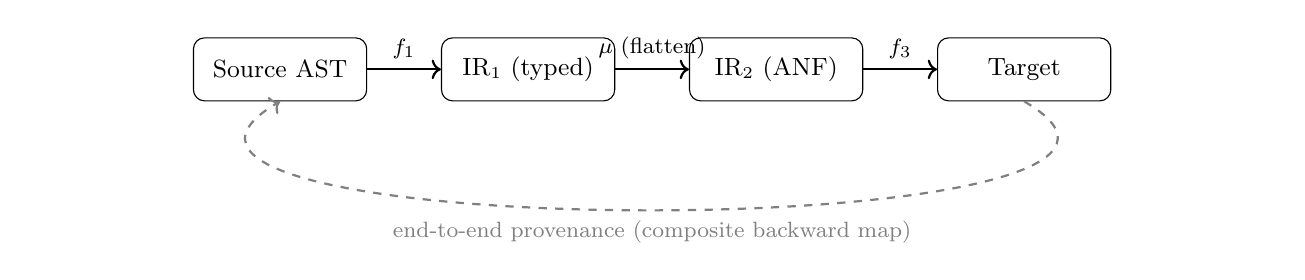
\begin{tikzpicture}[
    box/.style={draw, rounded corners, minimum width=22mm, minimum height=8mm,
      font=\small},
    arr/.style={thick, ->},
    scale=0.9
  ]
  \node[box] (src) at (0,0) {Source AST};
  \node[box] (ir1) at (3.5,0) {IR$_1$ (typed)};
  \node[box] (ir2) at (7,0) {IR$_2$ (ANF)};
  \node[box] (tgt) at (10.5,0) {Target};

  \draw[arr] (src) -- node[above, font=\footnotesize] {$f_1$} (ir1);
  \draw[arr] (ir1) -- node[above, font=\footnotesize] {$\mu$ (flatten)} (ir2);
  \draw[arr] (ir2) -- node[above, font=\footnotesize] {$f_3$} (tgt);

  % Backward provenance
  \draw[arr, dashed, gray] (tgt.south) to[out=-30,in=-150]
    node[below, font=\footnotesize, text=gray] {end-to-end provenance
      (composite backward map)} (src.south);
\end{tikzpicture}
\end{center}

\subsection{Scope Management as Directed Container}

A typing context $\Gamma = (x_1 : A_1,\; x_2 : A_2(x_1),\;
x_3 : A_3(x_1, x_2))$ is a snoc-list, and the category of contexts and
substitutions is a directed container:
\begin{itemize}[nosep]
\item \textbf{Shapes}: contexts $\Gamma$ (lists of typed variable declarations).
\item \textbf{Positions at $\Gamma$}: well-typed terms in context $\Gamma$
  (or, more simply, de~Bruijn indices into $\Gamma$).
\item \textbf{Root} $o(\Gamma)$: the identity substitution.
\item \textbf{Shift} $\oplus$: substitution composition.
\item \textbf{Downarrow} $\Gamma \downarrow p$: the context reached by
  applying substitution~$p$.
\end{itemize}

The comonad structure gives weakening and substitution canonically.
The two colours reappear: colour~1 edges (term structure) preserve the
context; colour~2 edges (binding) shift the context via $\downarrow$.
The scope checker is the functor from the ``unscoped'' container (raw
syntax, all positions equivalent) to the ``scoped'' directed container
(positions carry de~Bruijn indices, binding edges shift them).

%% ===================================================================
\section{Summary}
%% ===================================================================

\begin{center}
\renewcommand{\arraystretch}{1.3}
\begin{tabular}{@{}lll@{}}
\hline
\textbf{Container theory} & \textbf{Compiler theory} & \textbf{Colour} \\
\hline
Outer position $p \in P_1(s_1)$ & Subterm slot & 1 (line) \\
Inner position $q \in P_2(v(p))$ & Binding slot & 2 (containment) \\
Container morphism $(u, f^\sharp)$ & Compilation pass & --- \\
\quad Forward $u$ & Syntax translation & shapes \\
\quad Backward $f^\sharp$ & Provenance / blame & positions \\
Snoc-list container $L$ & Context / telescope & 2 (binding spine) \\
$B \circ L$ (branching $\circ$ snoc) & Syntax with telescopic binders & both \\
$L \circ B$ (snoc $\circ$ branching) & Sequence of IR passes & both \\
$\mu$ for $B \circ L$ & Telescope concatenation (ANF) & merge $2 \to 1$ \\
Free monad $\Free(C)$ & Multi-pass IR (unfixed depth) & all \\
Directed container & Scoped syntax + substitution & --- \\
\hline
\end{tabular}
\end{center}

The diagram on the first page---a tree with two colours of edge, one
drawn as lines and the other as containment---is the picture of container
composition. When the nesting is self-similar and unbounded, it is the
free monad. In compiler theory, the two colours are always present: one
for term structure, one for binding. Seeing them as container composition
makes the structure of compilation passes, normal forms, and provenance
into consequences of the functorial machinery rather than ad hoc
constructions.

\end{document}
